% This file was created by tikzplotlib v0.9.3.
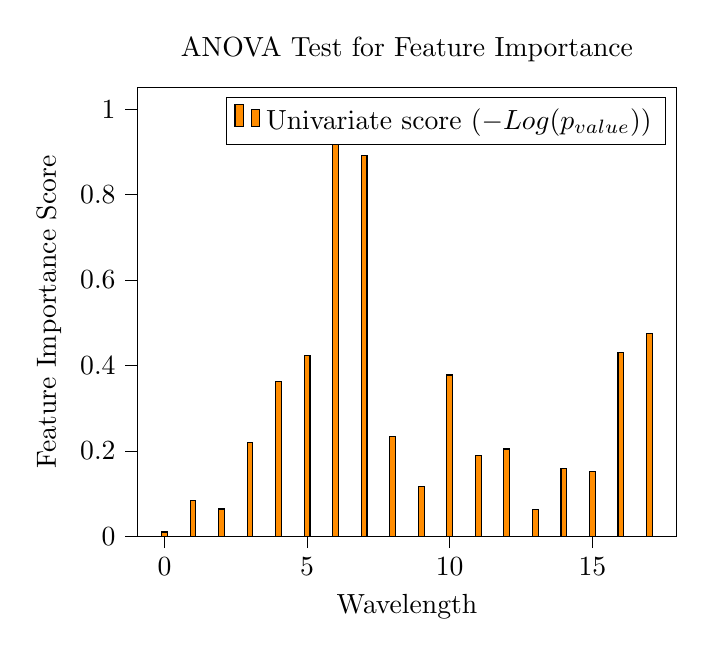
\begin{tikzpicture}

\definecolor{color0}{rgb}{1,0.549019607843137,0}

\begin{axis}[
tick align=outside,
tick pos=left,
title={ANOVA Test for Feature Importance},
x grid style={white!69.0196078431373!black},
xlabel={Wavelength},
xmin=-0.96, xmax=17.96,
xtick style={color=black},
y grid style={white!69.0196078431373!black},
ylabel={Feature Importance Score},
ymin=0, ymax=1.05,
ytick style={color=black}
]
\draw[draw=black,fill=color0] (axis cs:-0.1,0) rectangle (axis cs:0.1,0.00979463063771668);
\addlegendimage{ybar,ybar legend,draw=black,fill=color0};
\addlegendentry{Univariate score ($-Log(p_{value})$)}

\draw[draw=black,fill=color0] (axis cs:0.9,0) rectangle (axis cs:1.1,0.0828330157746437);
\draw[draw=black,fill=color0] (axis cs:1.9,0) rectangle (axis cs:2.1,0.0637002574950648);
\draw[draw=black,fill=color0] (axis cs:2.9,0) rectangle (axis cs:3.1,0.219817788760313);
\draw[draw=black,fill=color0] (axis cs:3.9,0) rectangle (axis cs:4.1,0.36209047994037);
\draw[draw=black,fill=color0] (axis cs:4.9,0) rectangle (axis cs:5.1,0.423271089223967);
\draw[draw=black,fill=color0] (axis cs:5.9,0) rectangle (axis cs:6.1,1);
\draw[draw=black,fill=color0] (axis cs:6.9,0) rectangle (axis cs:7.1,0.892650492971745);
\draw[draw=black,fill=color0] (axis cs:7.9,0) rectangle (axis cs:8.1,0.233197068216636);
\draw[draw=black,fill=color0] (axis cs:8.9,0) rectangle (axis cs:9.1,0.116086172011005);
\draw[draw=black,fill=color0] (axis cs:9.9,0) rectangle (axis cs:10.1,0.377641923013311);
\draw[draw=black,fill=color0] (axis cs:10.9,0) rectangle (axis cs:11.1,0.188684516124635);
\draw[draw=black,fill=color0] (axis cs:11.9,0) rectangle (axis cs:12.1,0.204252004618566);
\draw[draw=black,fill=color0] (axis cs:12.9,0) rectangle (axis cs:13.1,0.0622311976699345);
\draw[draw=black,fill=color0] (axis cs:13.9,0) rectangle (axis cs:14.1,0.159267618216081);
\draw[draw=black,fill=color0] (axis cs:14.9,0) rectangle (axis cs:15.1,0.150977567525683);
\draw[draw=black,fill=color0] (axis cs:15.9,0) rectangle (axis cs:16.1,0.431098080303937);
\draw[draw=black,fill=color0] (axis cs:16.9,0) rectangle (axis cs:17.1,0.473988114917983);
\end{axis}

\end{tikzpicture}
